\documentclass{beamer}
%\usepackage{mdwlist}
\usepackage{graphicx}

\usetheme{Hannover}

\usepackage{tikz}
\usetikzlibrary{shapes,arrows,shadows,fit}

\usepackage{listings}
\lstset{%
    language=Python,                   % choose the language of the code
    basicstyle=\ttfamily,       % the size of the fonts that are used for the code
    keywordstyle=\color{blue},
    stringstyle=\color{orange},
    numbers=none,                   % where to put the line-numbers
    numberstyle=\footnotesize,      % the size of the fonts that are used for the line-numbers
    stepnumber=2,                   % the step between two line-numbers. If it's 1 each line will be numbered
    numbersep=5pt,                  % how far the line-numbers are from the code
    backgroundcolor=\color{white},  % choose the background color. You must add \usepackage{color}
    showspaces=false,               % show spaces adding particular underscores
    showstringspaces=false,         % underline spaces within strings
    showtabs=false,                 % show tabs within strings adding particular underscores
    frame=none,                   % adds a frame around the code
    tabsize=2,	                    % sets default tabsize to 2 spaces
    captionpos=b,                   % sets the caption-position to bottom
    breaklines=true,                % sets automatic line breaking
    breakatwhitespace=false,        % sets if automatic breaks should only happen at whitespace
}

% Uncomment this if you use the notes
\usepackage{pgfpages}
% Comment these both out for no notes
%\setbeameroption{show notes}                  % Notes on separate page
%\setbeameroption{show notes on second screen} % Page is larger to include notes

% Removes the silly controls
\setbeamertemplate{navigation symbols}{}
% Put slide numbers at the bottom
\setbeamertemplate{footline}[page number]

\title[ServiceSniffer]{Team 11 --- ServiceSniffer}
%\subtitle{}
\author[Team 11]{
    Justin Courts \and
    Philip Cristiano \and\\
    Charles Rumford \and
    Thomas Wambold}
\institute[CS492]{CS492\\Drexel University\\\url{http://servicesniffer.net}}
\date{May 18, 2010}

% Do this for notes.
% \note[item]{Baz}

% To include a logo, seems to not work right with all themes
%\logo{\includegraphics[width=3cm]{../logo}}

%%% Tikz stuff %%%
% Style for UML Class with attributes and methods
\tikzstyle{umlclass} = [
    rectangle, rectangle split, rectangle split parts=3,
    % This makes a nice gradient
    top color=white, bottom color=blue!30, draw=blue!50!black!100,
    drop shadow, rounded corners,
    node distance = 4cm, text width = 35mm, font={\scriptsize}]

% Line styles
\tikzstyle{hasa} = [draw, ->, >=open diamond]
\tikzstyle{ownsa} = [draw, ->, >=diamond]
\tikzstyle{isa} = [draw, ->, >=open triangle 45]

\newcommand{\umlclass}[5][,]{
    \node [umlclass,#1] (#2) {
        \textbf{#3}
        \nodepart{second}
        #4
        \nodepart{third}
        #5
    };
}

\newcommand{\umlattr}[3]{
    $#1$\textbf{#2}: \textit{#3}
}
\newcommand{\umlmethod}[4]{
    $#1$\textbf{#2}({#3}): \textit{#4}
}
\newcommand{\umlarg}[2]{\textit{#1} #2}

\newcommand{\umlrelation}[6][-|]{
    \path [#3] (#2) #1 (#4)
        node [very near start, auto=right] {#5}
        node [very near end, auto=left] {#6};
}
%% End tikz stuff %%%

\begin{document}

%------------------------------------------------------------------------------

\begin{frame}
    \begin{figure}
        \centering
        \includegraphics[width=.35\textwidth]{../logo}
    \end{figure}
    \vspace{-10mm}
    \titlepage
    \note[item]{Justin}
    \note[item]{ServiceSniffer is an application layer protocol analysis tool
                currently focused on web services}
\end{frame}

%------------------------------------------------------------------------------
\section{Attacks!}

\begin{frame}{Attack Methods}
    \begin{itemize}
        \item Denial of Service
        \item Replay Attacks
        \item Information Leakage through web page source code and error
              messages
        \item SQL Injection
    \end{itemize}
    \note[item]{Justin}
    \note[item]{These are common problems web servers have to deal with today.
                Most of these problems have solutions, but as we'll see, using
                web services reintroduces these problems.}
\end{frame}

%------------------------------------------------------------------------------

\begin{frame}{Web Services}
    \begin{itemize}
        \item Web Services:  Typically client/server communication over HTTP in
              XML, frequently used protocols being SOAP, REST, WSDL, and UDDI.
    \end{itemize}
    \note[item]{Justin}
    \note[item]{Brief definition of web services and some associated
                protocols/specs}
    \note[item]{Web Services:  Typically Client/Server communication over HTTP
                in XML}
    \note[item]{SOAP:  A protocol web services communicate with}
    \note[item]{REST:  Web service model using HTTP commands for object
                interaction}
    \note[item]{WSDL:  XML-based model for describing web services}
    \note[item]{UDDI:  XML-based registry for web services}
\end{frame}

%------------------------------------------------------------------------------

\begin{frame}{New Old Problems}
    \begin{itemize}
        \item Old methods + Data encapsulating = Same problems but no solutions
        \item \textbf{XML} Denial of Service
        \item \textbf{SOAP Request} Replay Attacks
        \item Information Leakage through \textbf{server responses and error
              messages}
        \item SQL Injection
    \end{itemize}
    \note[item]{Justin}
    \note[item]{XML DoS by very deeply nesting XML tags, which is heavily CPU
                and/or memory intensive, or oversized request data}
    \note[item]{Replay Attacks allow DoSing as well as performing transactions
                that can't safely be repeated.}
    \note[item]{Information leakage can give up server names, all possible
                variables to submit, data formats for abuse, etc.}
    \note[item]{SQL Injection can, just like with webforms, be used to execute
                undesired SQL commands.  Little Bobby Tables over SOAP.}
    \note[item]{Problems previously solved are now reborn, and we're currently
                ill-equipped to handle them}
    \note[item]{All of the above are vulnerabilities the NSA, among others,
                sees as troublesome at best and destructive at worst.}
\end{frame}

%------------------------------------------------------------------------------

\begin{frame}{Brief project overview}
    \begin{itemize}
        \item Goals of ServiceSniffer:
        \begin{itemize}
            \item Help solve application layer issues
            \item Allow for and encourage future development
            \item Expose result sets through a GUI and a CLI
        \end{itemize}
    \end{itemize}
    \note[item]{Justin}
    \note[item]{Goal of ServiceSniffer is to help solve these problems}
    \note[item]{Application layer network/protocol analyzer}
    \note[item]{Highly extensible for future development}
    \note[item]{GUI for active users; scriptable CLI for automation and
                consumption}
\end{frame}

%------------------------------------------------------------------------------

\begin{frame}{Other products}
    \begin{itemize}
        \item \textbf{Wireshark} - Cumbersome, manual process 
        \item \textbf{Snort} - Lower layer NIDS
        \item \textbf{Nagios} - Lower layer notification framework
    \end{itemize}
    \note[item]{Phil}
    \note[item]{\textbf{Wireshark}:  Data is available to determine this data,
                but it would need to be gotten manually.  Wireshark not
                designed for these tasks}
    \note[item]{\textbf{Snort}:  Way too clunky and bloated to use, and
                requires a domain-specific language to be learned just to use
                it}
    \note[item]{\textbf{Nagios}:  Lower layer notification framework designed
                more for event triggers than analysis}
\end{frame}

%------------------------------------------------------------------------------

\begin{frame}{XML DoS}
    \begin{itemize}
        \item \textbf{Very} large payloads
        \item XML Bombs
        \item Recursive content
        \item Malicious external entities
        \item Malicious DTDs
        \item etc.
    \end{itemize}
    \note[item]{Phil}
    \note[item]{Very large payloads: An incredible amount of data to try to
                parse/store - heavy memory}
    \note[item]{XML Bombs:  Smallish request with exponentially growing
                expansions (a='foo'; b=a+a; c=b+b; d=c+c; etc.) heavy
                CPU/memory}
    \note[item]{Recursive content: eats CPU/memory}
    \note[item]{Malicious entities/DTDs: tries to get the server to do
                something it shouldn't}
\end{frame}

%------------------------------------------------------------------------------

\begin{frame}{Wireshark Demo}
    \begin{figure}
        \centering
        \includegraphics[width=.75\textwidth]{gfx/wireshark}
    \end{figure}
    \begin{itemize}
        \item Even with filtering, using Wireshark can be like finding a needle
            in a haystack.
    \end{itemize}
    \note[item]{Phil}
    \note[item]{In Wireshark, in order to find XML/SOAP requests which are a
                certain percentage larger than the current average isn't
                possible}
    \note[item]{You also can't walk through the WSDL for the web service, nor
                invoke it}
\end{frame}

%------------------------------------------------------------------------------
\section{Demo}

\begin{frame}{Demo}
    \begin{itemize}
        \item XML DoS Detection
        \item WSDL and web-service invocation
    \end{itemize}
    \note[item]{Phil}
    \note[item]{Tom's going to show you a little bit about ServiceSniffer, and
                go through two use cases:  finding XML DoS attacks and web
                service invocations using their WSDL definition.}
    \note[item]{Demo1: XML DoS}
    \note[item]{Demo2: WSDL invocation}
    \note[item]{Other uses, like debugging and discovering new web services on
                your machine}
\end{frame}

%------------------------------------------------------------------------------

\section{Design}

\begin{frame}{Design Overview}
    \begin{itemize}
        \item Modular approach for component independence and extensibility
        \item Modules:
        \begin{itemize}
            \item Capture
            \item System Kernel
            \item Processors/Filters
            \item Interfaces
        \end{itemize}
    \end{itemize}
    \note[item]{Charles}
\end{frame}

%------------------------------------------------------------------------------

\begin{frame}{System Design UML}
    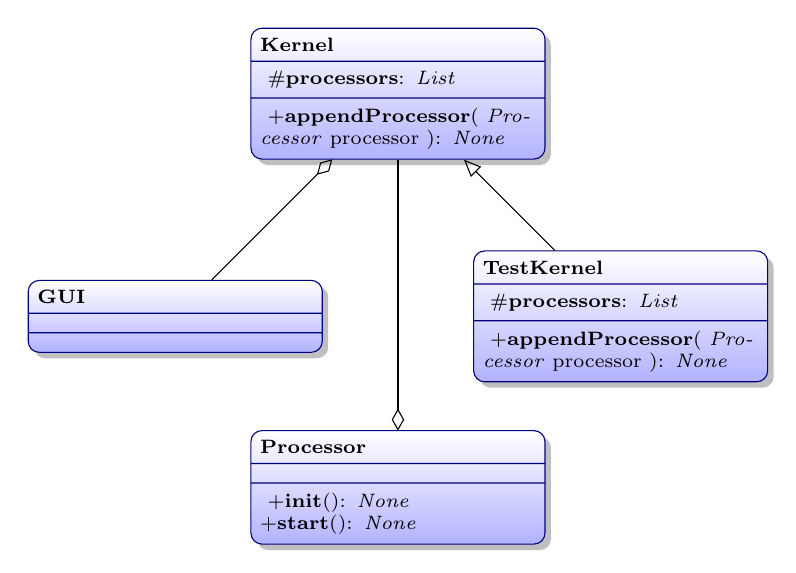
\begin{tikzpicture}
        \umlclass{kernel}{Kernel}{
        \umlattr{\#}{processors}{List}
        }{
            \umlmethod{+}{appendProcessor}{
                \umlarg{Processor}{processor}
            }{None}
        } 

\umlclass[below left of=kernel]{gui}{GUI}{ }{ }

\umlclass[below right of=kernel]{testKernel}{TestKernel}{
        \umlattr{\#}{processors}{List}
        }{
            \umlmethod{+}{appendProcessor}{
                \umlarg{Processor}{processor}
            }{None}
        }

\umlclass[below of=kernel,yshift=-10mm]{processor}{Processor}{
        }{
            \umlmethod{+}{init}{}{None}\\
            \umlmethod{+}{start}{}{None}
        }

        \umlrelation[--]{kernel}{hasa}{processor}{}{}
        \umlrelation[--]{gui}{hasa}{kernel}{}{}
        \umlrelation[--]{testKernel}{isa}{kernel}{}{}
    \end{tikzpicture}

    \note[item]{Charles}
    \note[item]{\textbf{Capture}: Collects traffic, does TCP stream
                reconstruction, and adds some meta-information to the data
                which can be useful later, like timestamping}
    \note[item]{\textbf{System Kernel}: Chain together processors and filters
                and act as the central hub for the system}
    \note[item]{\textbf{Processors/Filters}: Do the transformation and analysis
                of the traffic/data}
    \note[item]{\textbf{Interfaces}: GUI for interactive user; CLI for
                scriptable interface}
    \note[item]{They're all tied together through the System Kernel, but each
                unit is modular and can be pulled out and replaced with any
                module that implements the same interface}
\end{frame}


%------------------------------------------------------------------------------

\begin{frame}{Design Overview}
    \framesubtitle{Capture}
    \begin{figure}
        \vspace{-2em}
        \centering
        \includegraphics[width=.75\textwidth]{gfx/newdataflow}
        \vspace{-1em}
    \end{figure}
    \begin{itemize}
        \item{Uses LibPCAP and LibNIDS}
        \item{Ability to process live network traffic and Pcap files}
        \item{Ability to dump live network traffic for later processing}
    \end{itemize}
    \note[item]{Charles}
    \note[item]{libnids is used to reconstruct TCP streams.}
    \note[item]{We created a Python wrapper which we will contribute back to
        the community.}
    \note[item]{More useful to analyze data offline than live.}
\end{frame}

%------------------------------------------------------------------------------

\begin{frame}{Design Overview}
    \framesubtitle{System Kernel}
    \begin{figure}
        \vspace{-2em}
        \centering
        \includegraphics[width=.75\textwidth]{gfx/newdataflow}
        \vspace{-1em}
    \end{figure}
    \begin{itemize}
        \item{Central core to the system}
        \item{Control flow of information to the rest of the system}
        \item{Interacts with input, processing and interfaces}
    \end{itemize}
    \note[item]{Charles}
    \note[item]{Kernel coordinates data flow through other processors.}
    \note[item]{Responsible for starting and stopping the system.}
\end{frame}

%------------------------------------------------------------------------------

\begin{frame}{Design Overview}
    \framesubtitle{Processors and Filters}
    \begin{figure}
        \vspace{-2em}
        \centering
        \includegraphics[width=.75\textwidth]{gfx/newdataflow}
        \vspace{-1em}
    \end{figure}
    \begin{itemize}
       \item{Ability to reduce the data being shown or processing}
       \item{Processors can determine useful information from web services}
    \end{itemize}
    \note[item]{Charles}
    \note[item]{Each filter/processor runs in its own OS process.}
    \note[item]{This takes advantage of multi-core systems.}
    \note[item]{Filters/processors can be chained together in a similar manner
        to UNIX pipes.}
    \note[item]{They communicate with each other through shared message
        queues.}
\end{frame}

%------------------------------------------------------------------------------

\begin{frame}{Design Overview}
    \framesubtitle{Interfaces}
    \begin{figure}
        \vspace{-2em}
        \centering
        \includegraphics[width=.75\textwidth]{gfx/newdataflow}
        \vspace{-1em}
    \end{figure}
    \begin{itemize}
        \item{User control of the system}
        \item{Ability to control filters and processors}
        \item{Allows for different interfaces}
    \end{itemize}
    \note[item]{Charles}
    \note[item]{Currently available GUI interface.}
    \note[item]{GUI allows one to use a subset of the functionality easily.}
    \note[item]{Library-based CLI interface allows users to manipulate data and
        automate report generation easily, as well as allow consumption of the
        output by other programs.}
\end{frame}

%------------------------------------------------------------------------------
\section{Design Considerations}

\begin{frame}[fragile]{Example Library Configuration}
    \begin{lstlisting}
from servicesniffer import Kernel

k = Kernel()
# Load input packets from this pcap file
k.append_processor(Capture(PCAP_INPUT))
# Filter by IP addresses
k.append_processor(
    IPFilter([
        ('192.168.1-5.*:*', '72.14.204.99:80')
    ]))
# Only capture SOAP packets
k.append_processor(ProtocolFilter(SOAP))
# Send output to CLI
k.append_processor(ConsoleOutput())
k.start()
    \end{lstlisting}
    \note[item]{Justin}
    \note[item]{Along with the GUI Tom showed, we have a library-based
                interface which allows for scriptable automation and
                consumption of our system's output}
    \note[item]{We designed our system to not require a domain specific
                language and instead developed ServiceSniffer as a Python
                library similar to scientific computing packages like SciPy,
                MatPlotLib, and NumPy.}
    \note[item]{Similar to these packages, all of Python is available to the
                user of the library.}
\end{frame}

%------------------------------------------------------------------------------

\begin{frame}{Extensibility}
    \begin{itemize}
        \item New protocols --- XMPP or non-web service protocols
        \item New reports --- Custom aggregate data
        \item New interfaces --- Mobile Client, Application Plug-ins
        \item New filters/processors --- Protocol specific processing
    \end{itemize}
    \note[item]{Justin}
    \note[item]{Each filter/processor is decoupled from the rest of the
        system.}
    \note[item]{Users can create new processors without touching the rest of
        the code base.}
\end{frame}

%------------------------------------------------------------------------------

\begin{frame}{Alternative designs}
    \begin{itemize}
        \item Why Python and not C, Java, etc.?
        \item Process-based filtering/processing vs. Integrated
        \item Message passing (Queues) vs. Threading
    \end{itemize}
    \note[item]{Justin}
    \note[item]{Python allows a rapid development pace, has libraries in place
                to accomplish networking tasks, and easily interfaces with C
                libraries.}
    \note[item]{Process-based filtering allows for filters to be written in any
                language.}
    \note[item]{Message passing was chosen over threading to avoid common
                concurrency issues like deadlock as well as to decouple the
                system.}
\end{frame}

%------------------------------------------------------------------------------
\section{Tools \& Testing}

\begin{frame}{Software Development Tools}
    \begin{itemize}
        \item Version Control:  Git
        \item Development Environment:  VirtualEnv
        \item Unit Testing:  Nose
        \item Project Management:  Experimented with Basecamp, Trac, and Bugs
              Everywhere
    \end{itemize}
    \note[item]{Phil}
    \note[item]{
                Tried multiple tools, spent more time on them then coding. 
                Most of coding done in a group + tested processors meant fewer bugs
               }

\end{frame}

%------------------------------------------------------------------------------

\begin{frame}{Testing}
    \begin{itemize}
        \item Nose: code coverage
        \item 88\% code coverage on the library
        \item Test cases for each filter/processor.
    \end{itemize}
    \note[item]{Phil}
    \note[item]{Nose is a library around Python's \texttt{unittest} library.}
    \note[item]{Message passing allows for easy testing of each
        filter/processor, since we can feed in testing data, and check output.}
\end{frame}

%------------------------------------------------------------------------------
\section{Conclusion}

\begin{frame}{Wrap-up}
    \begin{itemize}
        \item Application layer service analyzer currently focused on web
            services (SOAP, XML, WSDL, UDDI)
        \item Helps find:
        \begin{itemize}
            \item XML Denial of Service
            \item Information Leakage through WSDL/error messages
            \item Replay Attacks
            %\item SQL Injection
        \end{itemize}
        \item Reports and Statistics
    \end{itemize}
    \note[item]{Phil}
\end{frame}

%------------------------------------------------------------------------------

\begin{frame}{Questions?}
    \begin{itemize}
        \item See our website at \url{http://servicesniffer.net}
        \item Can send questions to \url{list@servicesniffer.net}
    \end{itemize}
    \note[item]{Tom}
\end{frame}

%------------------------------------------------------------------------------

\end{document}
